\chapter{Question 1}
\section{Questions}
Given is the function $f$ determined by
$f(x) = \cosh(x) = \frac{e^x + e^{-x}}{2}$.
\begin{enumerate}
  \item Find the natural domain $D$ of the given functional expression.
  \item Look at potential symmetry properties of the function.
  \item Find the roots of the function, that is, the points $x \in D$ where
  $f(x) = 0$.
  \item Asymptotic analysis: check for the existence of horizontal and vertical
  asymptotes.
  \item Investigate the behaviour of the first derivative.
  \item Investigate the behaviour of the second derivative.
  \item Collect the results in a table, and determine the type of the critical
  points.
  \item Finally, sketch the graph of $f$, using the previous table as a
  guideline.
\end{enumerate}

\section{Solutions}
\begin{enumerate}
\item Natural domain $D$ is goverend by $e^x$ and $e^{-x}$. As these can take
any real number, $D: x \in \mathbb{R}$.

\item Symmetrical properties:
\begin{enumerate}
  \item Function never dips below $x$ axis, so any symmetry (if present)
  \emph{must} be about the $y$ axis.

  \item For vertical symmetry, $f(x) = f(-x)$:
  \begin{align}
    f(x) &\stackrel{?}{=} f(-x) \\
    \frac{e^x + e^{-x}}{2} &\stackrel{?}{=} \frac{e^{-x} + e^{x}}{2} \\
    e^x + e^{-x} &\stackrel{?}{=} e^{-x} + e^{x} \\
  \end{align}
  $\therefore$ $f$ \emph{is} symmetrical about the $y$ axis.

  \item $f(0) = \frac{e^0 + e^{-0}}{2} = 1$, and is likely a minimum because
  throwing larger values for $x$ in produces larger numbers.
\end{enumerate}

\item $f(x) = 0$ iff $e^x + e^{-x} = 0$. As both $e^x$ and $e^{-x}$ are
strictly positive), they will always sum to a strictly positive number,
therefore $f(x) \neq 0$, so no real roots. This ties closely with the previous
part, $f(x) \geq 1$, never touching the $x$ axis.

\item $e^x$ dominates the function as $x \to \pm\infty$, as $x \to +\infty$,
$f(x) \to \infty$ even faster. This is also true of $x \to -\infty$ due to the
symmetry of $f$, so there are no asymptotes.

\item First derivative of $\cosh x$:
\begin{align}
  \cosh x &= \frac{e^x + e^{-x}}{2} \\
    &= \frac{1}{2} e^x + e^{-x} \\
  \left(\cosh x\right)' &= \frac{1}{2} e^x - e^{-x}
  \intertext{from looking on Wikipedia, this is $\sinh x$}
  \left(\cosh x\right)' &= \sinh x
  \intertext{Roots of $\sinh x$}
  0 &= \frac{1}{2} e^x - e^{-x} \\
    &= e^x - e^{-x}
  \intertext{Let $x=0$}
  0 &= 1-1 \label{eq:q1_critical}
\end{align}
Therefore one root exists at $x=0$. As seen in (b)(iii), this is a minimum
because of the "larger number test". This can be demonstrated in the second
derivative test below.

\item Second derivative of $\cosh x$. \\
This is the same as the first derivative of $\sinh x$:
\begin{align}
  \sinh x &= \frac{1}{2} e^x - e^{-x} \\
  \left(\sinh x \right)'
    &= \frac{e^x + e^{-x}}{2} \\
    &= \cosh x
\end{align}
Ah! Some interesting ring behaviours! With no roots for $(\cosh x)''$, and that
$(\cosh x)'' \geq 1$ we can infer that $\cosh x$ has a minimum at $x=0$ given
in \eqref{eq:q1_critical}.

\item Tabulating this sort of stuff in \LaTeX really sucks. Please accept the
logical ordering of the investigations in lieu of a table.

\item Plotting of $\cosh x$ in Mathematica with the following code: \\
\texttt{Plot[Sinh[x], \{x,-10,10\}, ImageSize $\to$ Large]} gives the graph in
figure \ref{fig:q1_plot} on page \pageref{fig:q1_plot}.
\begin{figure}[!ht]
  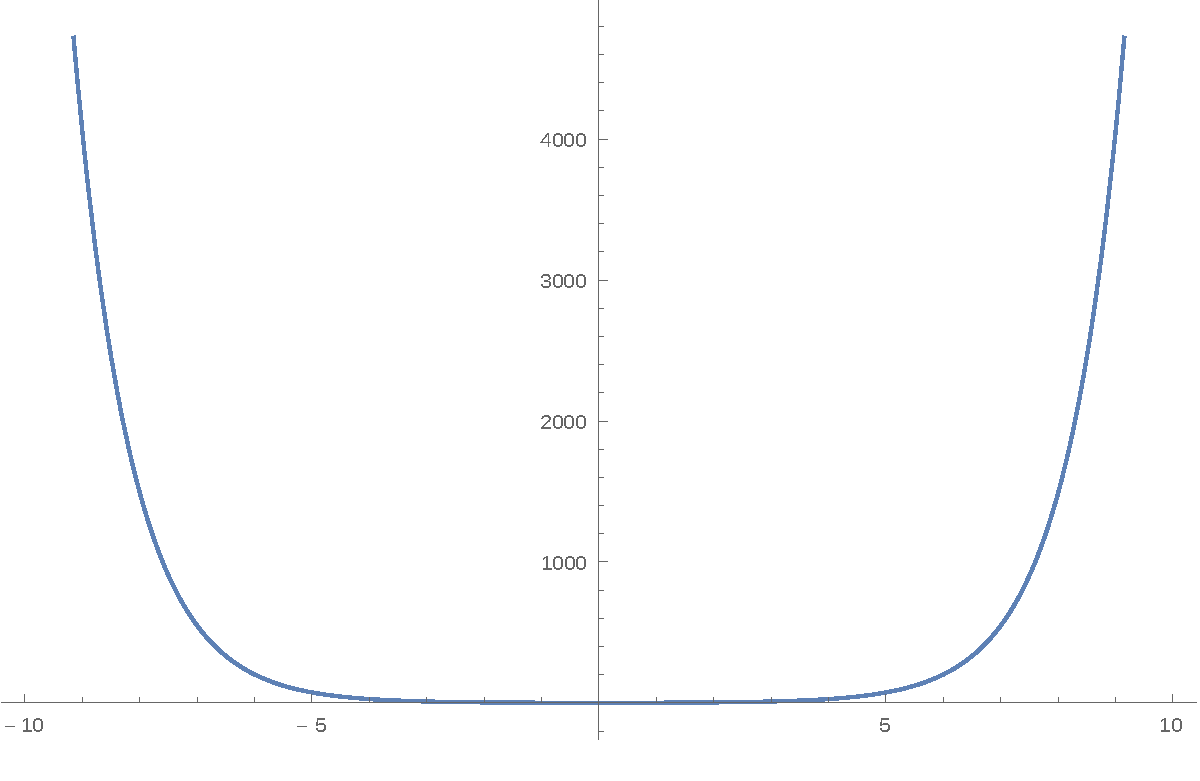
\includegraphics[width=\linewidth]{solutions/q1/plot.pdf}
  \caption{Plot of $\cosh x$}
  \label{fig:q1_plot}
\end{figure}
\end{enumerate}
